\documentclass{article}

\title{Metodi Numerici per l'Informatica}
\author{Anthony}
\date{18 apr 2023}

\usepackage{amssymb}
\usepackage{amsmath}
\usepackage{graphicx}

\newcommand*{\horzbar}{\rule[.5ex]{2.5ex}{0.5pt}}
\begin{document}
    \maketitle
    \section{Principal Component}
        Consideriamo i seguenti dati che vivono in $\mathbb{R}^2$:
        \begin{center}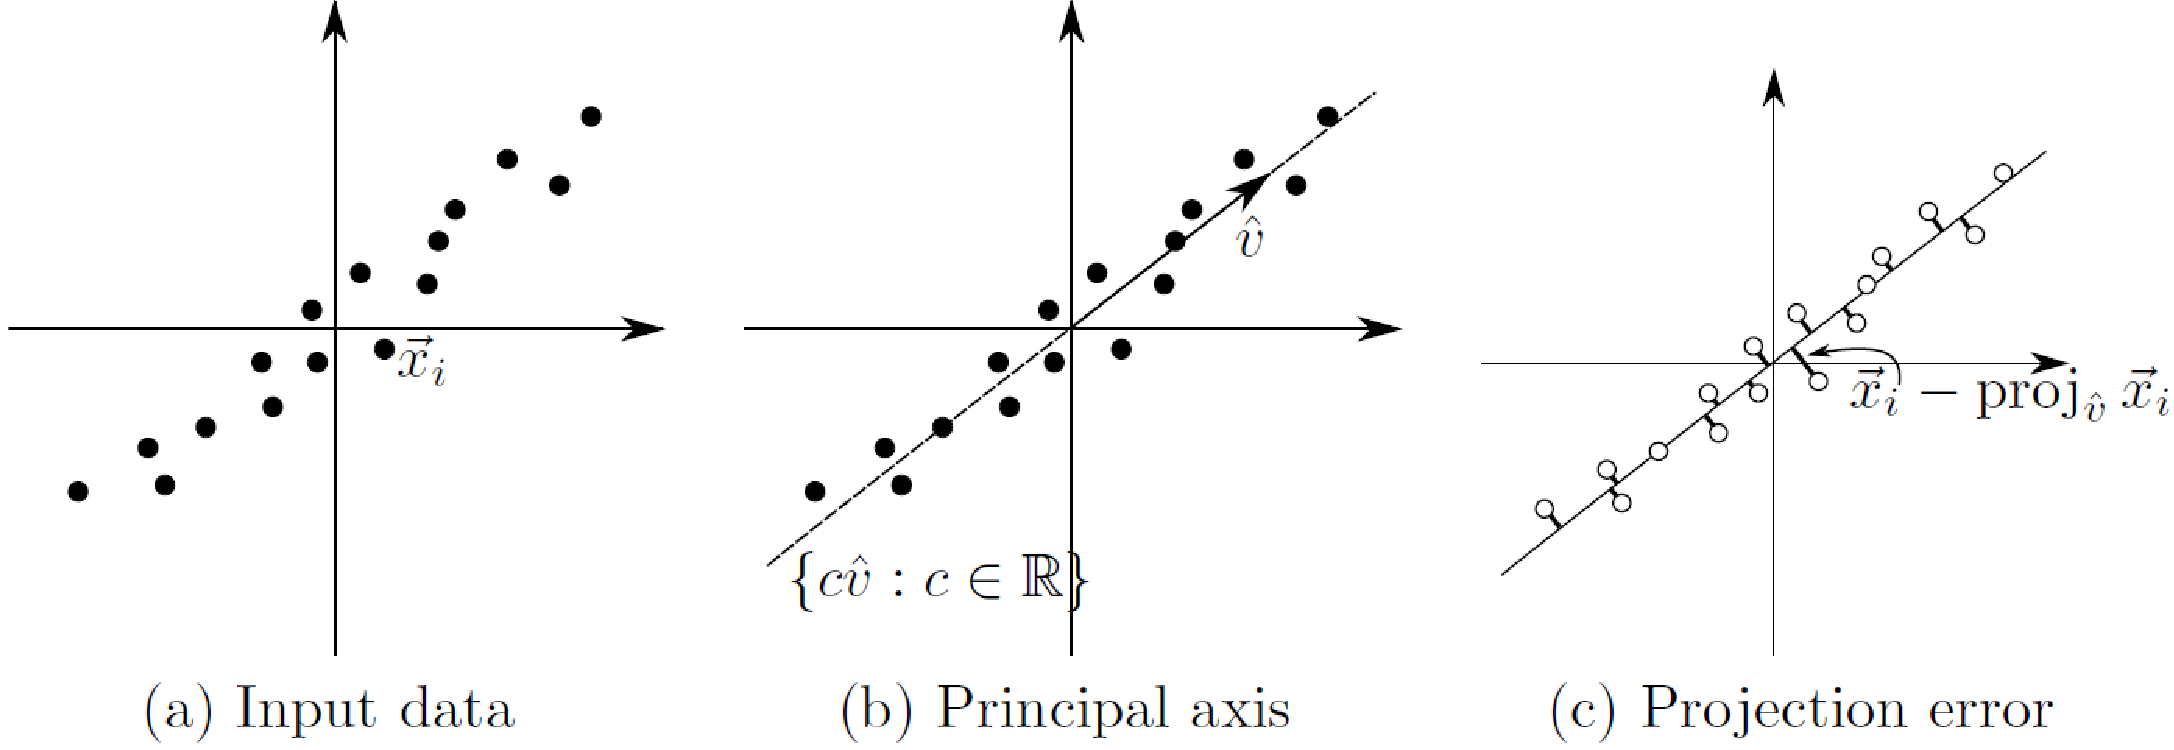
\includegraphics[width=12cm]{dati_r2.png}\end{center}
        Vogliamo trovare il vettore $\mathbf{v}$ tale che, per ogni data point $\mathbf{x}_i$, esso può essere scritto come:
            \[\mathbf{x}_i = c_i\mathbf{v}\]
        In altre parole, la distanza di ogni punto dalla retta misurata lungo la componente ortogonale della retta stessa 
        deve essere più piccola possibile. Vogliamo minimizzare tale somma delle distanze.
        \paragraph{Un'altra prospettiva} Supponiamo di avere $n$ punti nella matrice 
        $\mathbf{X} \in \mathbb{R}^{d \times n}$:
        \begin{center}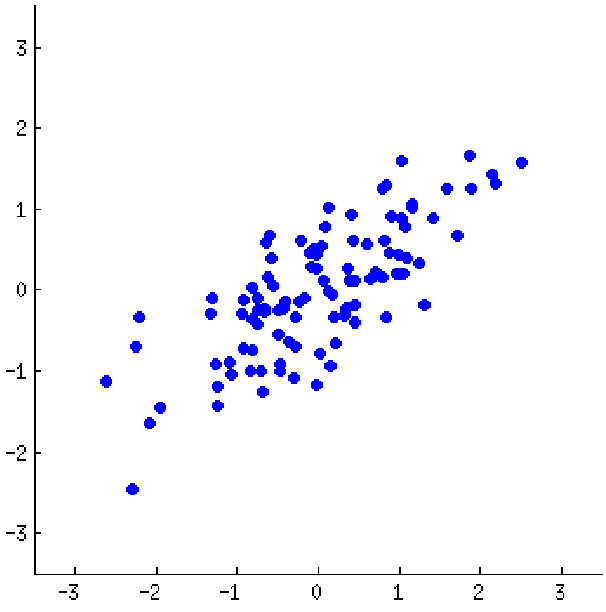
\includegraphics[width=5cm]{points.png}\end{center}
        Vogliamo approssimare i punti della matrice $\mathbf{X}$ in una matrice con meno dimensioni $\mathbf{\tilde{X}} \in \mathbb{R}^{k \times n}$
        con $k \ll d$. 
        \[ \mathbf{X}^T = \begin{pmatrix}
            \horzbar & \mathbf{x}_1^T & \horzbar \\
            & \vdots & \\
            \horzbar & \mathbf{x}_n^T & \horzbar
        \end{pmatrix} \approx
        \begin{pmatrix}
            - & \mathbf{x}_1^T & - \\
            & \vdots & \\
            - & \mathbf{x}_n^T & -
        \end{pmatrix} = \mathbf{\tilde{X}}^T\]
        Vogliamo quindi trovare le $k \leq d$ direzioni ortogonali con la maggior varianza. Esse spannano il sottospazio $k$-dimensionale 
        dei dati, poi vogliamo proiettare tutti i punti verso queste direzioni. Ciò induce a perdita di informazione, ma possiamo 
        farlo con la minor perdita possibile.
    \section{PCA}
        In generale, applicando PCA vogliamo identificare i $k \ll d$ assi per i quali, una volta proiettato il nostro dataset originale,
        minimizzano la perdita di informazione. Intuitivamente, gli assi che minimizzano la perdita di informazione sono ortogonali fra loro.
        Vogliamo quindi trovare la direzione $\mathbf{w}$ tale che:
        \begin{itemize}
            \item Minimizza l'errore di proiezione/ricostruzione
            \item Massimizza la varianza dei dati proiettati
        \end{itemize}
        Le due proprietà sono dunque equivalenti:
        \begin{center}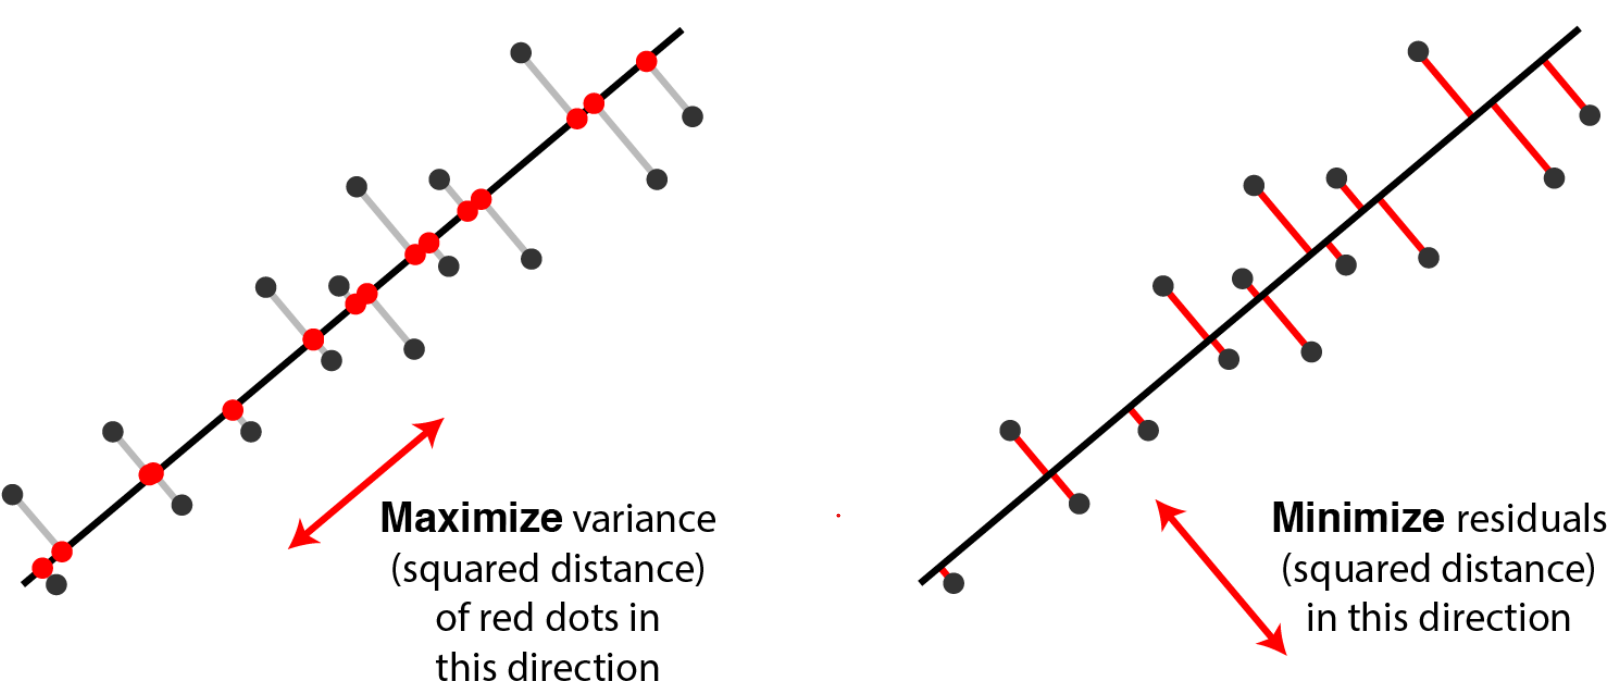
\includegraphics[width=9cm]{pca_minmax.png}\end{center}
        Ovvero, trovare l'asse che minimizza l'errore di proiezione è equivalente a trovare un asse che massimizza la varianza 
        dei dati.
        Possiamo pensare al PCA come a un cambio di base a meno dimensioni.
        \subsection{Notazione matriciale}
            Dati $\mathbf{x}_i$ i punti e $\mathbf{w}_i$ le assi, possiamo esprimere il problema in notazione 
            matriciale:
                \[\underbrace{\begin{pmatrix}
                    \horzbar & \mathbf{x}_1^T & \horzbar \\
                    & \vdots & \\
                    \horzbar & \mathbf{x}_n^T & \horzbar
                \end{pmatrix}}_{n\times d}
                \underbrace{
                    \begin{pmatrix}
                        | & & | \\
                        \mathbf{w}_1 & \dots & \mathbf{w}_k\\
                        | & & |
                    \end{pmatrix}}_{d \times k} =
                 \underbrace{\begin{pmatrix}
                    \horzbar & \mathbf{z}_1^T & \horzbar \\
                    & \vdots & \\
                    \horzbar & \mathbf{z}_n^T & \horzbar
                \end{pmatrix}}_{n \times k}\]
            Il prodotto interno ci consente di proiettare i punti nelle $k$ dimensioni del dataset originale. Questa 
            proiezione può avvenire solo se le dimensioni sono ortogonali tra di loro. \\
            Assumendo che $\mathbf{W}^T\mathbf{W} = \mathbf{I}$, per $k < d$ otteniamo:
            \[\mathbf{X}^T\mathbf{W} = \mathbf{Z}^T \quad \text{proiezione}\]
            \[\mathbf{X} \approx \mathbf{WZ} \quad \text{ricostruzione}\]
            Le due formule sono equivalenti:
            \begin{equation}
                \mathbf{X}^T\mathbf{W} = \mathbf{Z}^T
            \end{equation}
            \begin{equation}
               = \mathbf{X}^T\mathbf{WW}^T = \mathbf{Z}^T\mathbf{W}^T
            \end{equation}
            \begin{equation}
                =\mathbf{X}^T = \mathbf{Z}^T\mathbf{W}^T
            \end{equation}
            \begin{eqnarray}
                = \mathbf{X} = \mathbf{WZ}
            \end{eqnarray}
            Se $\mathbf{W}$ non è quadrata, presenta comunque $k$ colonne ortogonali. Una matrice $\mathbf{W} \in 
            \mathbb{R}^{d \times k}$ si dice \emph{semiortogonale} se $\mathbf{W}^T\mathbf{W} = \mathbf{I}_k$, ovvero il prodotto con 
            la sua trasposta è pari all'identità $k$-dimensionale. Poiché $\mathbf{W}$ non è una matrice quadrata, 
            l'operazione $\mathbf{WW}^T \approx \mathbf{I}_d$, ovvero non è necessariamente un'identità a $d$ dimensioni.
            Questo rende valida l'equazione di proiezione, tuttavia il passaggio $(3)$ non è più del tutto valido. In virtù 
            dell'approssimazione, possiamo dire $\mathbf{X} \approx \mathbf{WZ}$. Questo step è quello di ricostruzione poiché,
            data $\mathbf{WZ}$, ricostruiamo $\mathbf{X}$ effettuando una trasformazione lineare.
        \section{Risolvere PCA}
            Assumendo che abbiamo dei data points $\mathbf{X}$ centrati in zero, per un certo $\mathbf{w}$, la proiezione degli 
            $n$ punti su $\mathbf{w}$ è $\mathbf{X}^T\mathbf{w}$. La varianza da massimizzare è $\Vert \mathbf{X}^T\mathbf{w} \Vert_2^2$:
            \[(\mathbf{X}^T\mathbf{w})^T (\mathbf{X}^T \mathbf{w}) = \mathbf{w}^T \underbrace{\mathbf{XX}^T}_{\mathbf{C}}\mathbf{w}\]
            I cui $\mathbf{C} \in \mathbb{R}^{d \times d}$ è la matrice simmetrica di covarianza. Vogliamo massimizzare la covarianza, quindi 
            vogliamo risolvere il problema:
            \[\max_\mathbf{w} \mathbf{w}^T\mathbf{Cw} \quad \text{t.c. }\Vert \mathbf{w} \Vert^2_2 = 1\]
            La soluzione è proprio $\mathbf{w}$, l'autovettore principale di $\mathbf{C}$ per il principio min-max. Il suo autovalore 
            corrispondente è $\mathbf{w}^T\mathbf{Cw}$.
            \subsection{Trovare più componenti principali}
                Dopo aver risolto il problema: 
                \[\mathbf{w}_1 = \arg \max_\mathbf{w} \mathbf{w}^T\mathbf{Cw} \quad \text{t.c. }\Vert \mathbf{w} \Vert^2_2 = 1\]
                Per trovare la successiva direzione ortogonale possiamo aggiungere un nuovo vincolo al problema:
                \[\mathbf{w}_1 = \arg \max_\mathbf{w} \mathbf{w}^T\mathbf{Cw} \quad \text{t.c. }\Vert \mathbf{w} \Vert^2_2 = 1 \text{ e }\mathbf{w}_1^T\mathbf{w} = 0\]
                Ciò ci restituisce il secondo autovettore di $\mathbf{C}$. Iterando possiamo trovare i primi $k$ autovettori, che corrispondono 
                alle componenti principali di $\mathbf{C}$.
        \section{PCA come modello generativo}
            Dato un certo $\mathbf{W}$ che soddisfa le seguenti osservazioni su $\mathbf{X}$:
            \[\mathbf{X}^T\mathbf{W} = \mathbf{Z}^T \quad \text{proiezione}\]
            \[\mathbf{X} \approx \mathbf{WZ} \quad \text{ricostruzione}\]
            possiamo generare nuovi dati campionando $\mathbf{z_{new}} \in \mathbb{R}^k$ risolvendo:
            \[\mathbf{x_{new}} = \mathbf{Wz_{new}}\]
        

\end{document}